\section{Methodology and theory}
\label{sec:problem_description}

\subsection{Computer Vision - Image Segmentation}

For the acquired image data, appropriate image preprocessing can be applied. Under the premise of maintaining the integrity and quality of images, certain processing can be implemented to highlight the features intended for computer recognition and, to some extent, remove irrelevant features and noise. This enhances the accuracy of subsequent deep learning models.

Image segmentation is a critical step in image processing, aiming to divide the image into several meaningful regions for further analysis and processing. In models focusing on the yield rate of biological tissues, it is necessary to segment the biological sections into biological tissue and paraffin areas, emphasizing the biological tissue parts.

Common image segmentation algorithms include edge detection and threshold segmentation.

\subsubsection{Edge Detection}
For biological tissue sections, a crucial indicator of quality is the clarity of the section's edges. The integrity and continuity of the slice edges can reflect whether there are quality issues with the sample.

There are numerous algorithms for edge detection, such as Sobel, Laplacian, and Canny operators \cite{3.1}.

The \textbf{Sobel operator} is a first-order differential operator that can be used to detect image edges \cite{补充1}. Suppose there is a one-dimensional image $f(x)$, the relationship between its intensity and the pixel coordinate $x$ can be represented as shown in Figure 1. It can be observed in \autoref{fig:original_function} that the slope is the largest around x=2.2, indicating that there is a sudden change in image intensity (an edge exists) near this point. Taking its derivative gives the first-order derivative $f'(x)$, as shown in \autoref{fig:first_derivative}, where the absolute value of the derivative is the largest. The Sobel operator uses this characteristic to detect edges.

\begin{figure}[htbp]
    \centering
    \begin{minipage}[b]{0.32\textwidth}
        \centering
        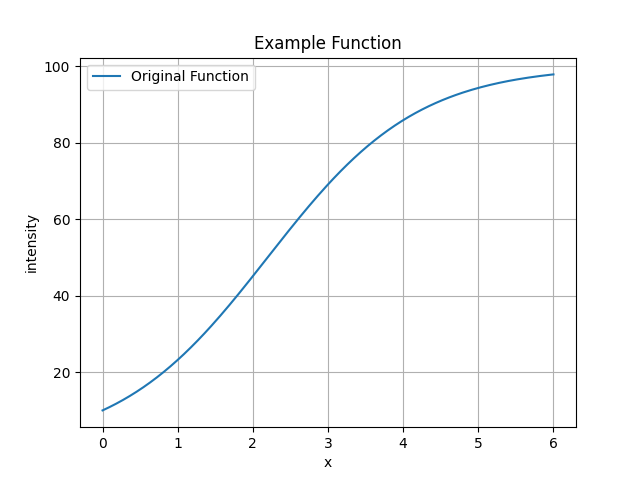
\includegraphics[width=\textwidth]{./fig/original_function.png}
        \caption{f(x)}
        \label{fig:original_function}
    \end{minipage}
    \begin{minipage}[b]{0.32\textwidth}
        \centering
        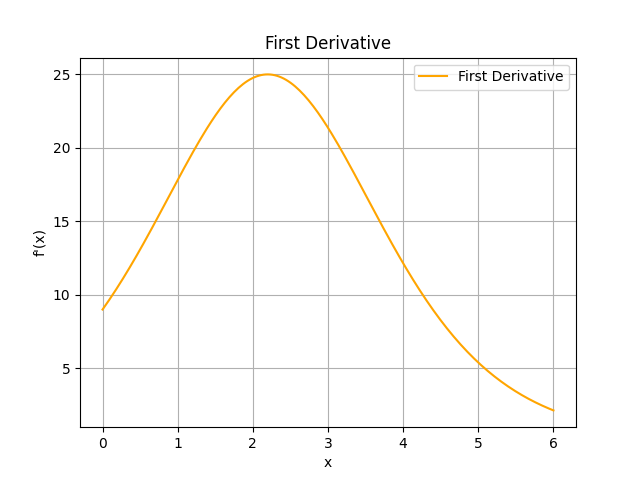
\includegraphics[width=\textwidth]{./fig/first_derivative.png}
        \caption{f'(x)}
        \label{fig:first_derivative}
    \end{minipage}
    \begin{minipage}[b]{0.32\textwidth}
        \centering
        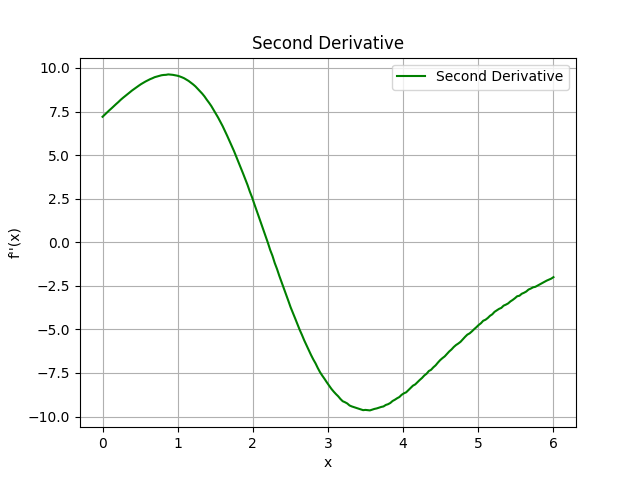
\includegraphics[width=\textwidth]{./fig/second_derivative.png}
        \caption{f''(x)}
        \label{fig:second_derivative}
    \end{minipage}
\end{figure}

The \textbf{Laplacian operator} is a second-order differential operator that performs well in edge detection of images. It is derived by taking the derivative of the Sobel operator once more. In 2D images, the Laplacian operator is defined as follows: 

\begin{equation} 
    \nabla^2 f = \frac{\partial^2 f}{\partial x^2} + \frac{\partial^2 f}{\partial y^2} 
\end{equation} 

As shown in the figure above, taking the derivative of the first-order derivative results in the second-order derivative $f''(x)$, as shown in \autoref{fig:second_derivative}. It can be seen that around x=2.2, the second-order derivative is 0, which indicates that when the value of the Laplacian operator $\nabla^2 f$ is 0, there is a sudden change in image intensity, indicating the presence of an edge.

\textbf{Canny Operator}is a multi-stage differential operator that enhances the edge detection process by incorporating noise suppression, building on the initial computations similar to those used by the Sobel operator. Introduced by John F. Canny in 1986 \cite{3.2}, the Canny operator refines the results obtained from Sobel operator calculations through additional steps such as non-maximum suppression and hysteresis thresholding. These steps set thresholds to eliminate false edges from the image, resulting in more accurate edge detection.

In the chapter on \textit{Experimental Work/Analytical Investigation/Design}, experiments will be conducted on the collected image data using these three edge detection algorithms—Sobel, Laplacian, and Canny—to compare their effectiveness. This comparative analysis will help in identifying the most suitable method for edge detection in the context of tissue sectioning, where the clarity and precision of edges are vital for quality assessment. The results will guide the selection of the optimal algorithm to be integrated into the image processing pipeline, enhancing the capability of the system to accurately segment and analyze biological tissue sections.

\subsubsection{Theresold Segmentation}

Apart from edge detection, another method employed is threshold segmentation. This technique divides the image pixels into two categories: those above a certain threshold and those below it. It is particularly useful in situations where there is a significant grayscale difference between the target and the background in the image.

For specimens, a straightforward approach is to contrast the colors of the paraffin area and the biological tissue area (which is stained during preparation), and then separate them using threshold segmentation. Assuming the biological tissue is yellow and the paraffin is white, setting a threshold could isolate the white parts of the image, leaving behind the biological tissue.

Additionally, there are more sophisticated methods of threshold segmentation, such as the Otsu method used for fingerprint extraction. Implementing this method can significantly enhance the segmentation of biological tissues. Yue Yaru and Zhu Jialin in "Algorithm of fingerprint extraction and implementation based on OpenCV" have proposed an improved Otsu-based fingerprint extraction algorithm using OpenCV. This algorithm excels particularly under conditions of uneven illumination and blurred images, providing accurate, simple, and fast fingerprint extraction \cite{3.3}.

Comparisons and experiments related to these segmentation techniques will be conducted in the \textit{Experimental Work/Analytical Investigation/Design} chapter.

\subsection{Deep Learning}

\subsubsection{Convolutional Neural Networks (CNN)}

Convolutional Neural Networks (CNNs) are a type of deep learning model that are particularly effective at processing image data. They automatically learn spatial hierarchies of features through a series of convolutional layers without the need for manual feature extraction. A typical CNN model includes layers such as convolutional layers, pooling layers, and fully connected layers \cite{3.4}. The architecture of a CNN is illustrated below:


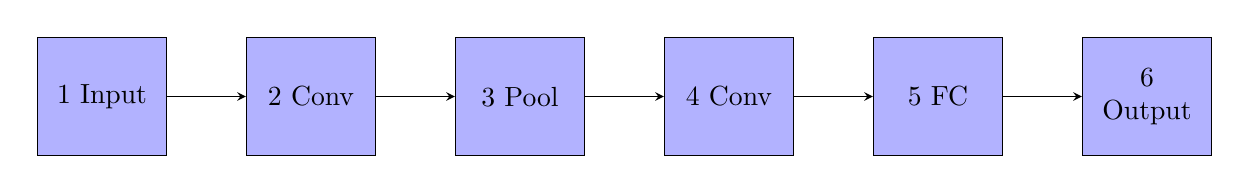
\begin{tikzpicture}[
    node distance=1cm and 0.5cm,
    block/.style={rectangle, draw, text width=4em, text centered, minimum height=15mm, fill=blue!30},
    arrow/.style={->,>=stealth}
]

% Define nodes in a matrix
\matrix [column sep=10mm, row sep=10mm] {
  \node (n1) [block] {1 Input}; & \node (n2) [block] {2 Conv}; & \node (n3) [block] {3 Pool} ;& \node
  (n4) [block] {4 Conv};    & \node (n5) [block] {5 FC};   & \node (n6) [block] {6 Output}; \\
};

% Connect nodes
\draw [arrow] (n1) -- (n2);
\draw [arrow] (n2) -- (n3);
\draw [arrow] (n3) -- (n4);
\draw [arrow] (n4) -- (n5);
\draw [arrow] (n5) -- (n6);
\end{tikzpicture}

In this model:

\textbf{Convolutional layers (Conv)}: These are the core layers of a CNN, responsible for feature extraction from images.

\textbf{Pooling layers (Pool)}: These serve to reduce the dimensionality of the feature maps, thereby decreasing the computational load.

\textbf{Fully connected layers (FC)}: These integrate the features extracted by the convolutional and pooling layers for classification or regression analysis, eventually leading to the output.

The typical method for training a CNN involves several key processes:

\begin{enumerate}
    \item \textbf{Forward Propagation:} Input data passes through each layer of the network until it reaches the output layer.
    \item \textbf{Loss Computation:} The network's output is compared to the actual labels using a loss function, such as cross-entropy loss, to calculate the difference.
    \item \textbf{Backpropagation:} The gradient of the loss function with respect to the network weights is computed.
    \item \textbf{Weight Update:} The network weights are updated using an optimization algorithm such as gradient descent or its variants like Adam or RMSprop, with the aim of minimizing the loss function.
\end{enumerate}

Once trained, the CNN can be employed to predict labels for new, unseen images. The distinctive feature of CNNs is their ability to automatically and efficiently learn features at different levels of abstraction, making them highly effective for tasks involving complex image data, such as medical image analysis, where accuracy and detail are paramount.

\subsubsection{Transfer Learning}

Indeed, for complex image tasks, constructing a simple CNN network is often insufficient. In such cases, transfer learning becomes essential. Transfer learning is a machine learning method that accelerates the training process by transferring knowledge from a pre-trained model to a new task. The core idea of transfer learning is to leverage knowledge from the source domain to aid learning in the target domain.

For CNN models, there are several approaches to transfer learning, such as fine-tuning and feature extraction: 

\textbf{Fine-tuning} involves adjusting the parameters of a pre-trained model to adapt it to a new task. This often includes retraining some of the convolutional layers along with the fully connected layers on the new data, which allows the model to fine-tune the features to the specific characteristics of the new dataset. 

\textbf{Feature extraction} involves using a pre-trained model as a fixed feature extractor, where only the fully connected layers are trained on the new data. In this approach, the convolutional layers retain their learned weights and act solely to extract features, which are then used by the newly trained classifier layers to perform tasks specific to the new dataset.

Commonly used pre-trained models include VGG, Inception, and others. These models have been extensively trained on large datasets like ImageNet, where the weights of various layers in the model have been optimized and can be effectively used for transfer learning.

Table 2 shows the number of parameters in models such as VGG16, VGG19 \cite{3.5}, InceptionV3 \cite{3.6}, Xception \cite{3.7}, etc. These models have a large number of parameters, allowing them to accurately extract features from complex images. The capability to leverage these well-trained models enables researchers and practitioners to achieve high performance on specific tasks without the need to train an entire network from scratch, saving both time and resources while maintaining high accuracy.

\begin{table}[htbp]
    \centering
    \caption{Comparison of CNN Models}
    \label{tab:model_comparison}
    \begin{tabular}{ccccc}
        \toprule
        \textbf{Model} & \textbf{VGG16} & \textbf{VGG19} & \textbf{InceptionV3} & \textbf{Xception} \\
        \midrule
        \textbf{Number of Parameters} & 138,357,544 & 143,667,240 & 23,851,784 & 22,910,480 \\
        \bottomrule
    \end{tabular}
\end{table}


\FloatBarrier






